\section{Metodología}

Ahora tenemos claro lo que queremos medir: 

En esta sección describimos paso a paso los procesos que caracterizan la reacción de trasferencia:

\begin{equation}
    ^{11} \text{Li} +  \text{d} \to  \text{t} + ^{10}  \text{Li} 
\end{equation}
desde el haz de litio 11, hasta la medida de las partículas lige

\subsection{Cinemática}

\subsubsection{Relatividad especial}

La relatividad especial nos permite estudiar la conservación de la energía y el momento usando los cuadrivectores. Definimos el 4-momento $P$ de una partícula de masa $m$ que se mueve a una velocidad $v$ de un sistema de coordenadas como:

\begin{equation}
    P = (p^0, \pn) = m \gamma (c,\vn) =\left( \frac{E}{c},\pn \right)   \label{Ec:01}
\end{equation}
La norma de un cuadrimomento cualquiera viene dado siempre por

\begin{equation}
    P^2  = - m^2 c^2  \label{Ec:02}
\end{equation}
Lo que antes era la ley de conservación de la energía y la ley de conservación del momento de cualquier fenómeno físico, ahora se puede condensar ahora en:

\begin{equation}
    \sum P_{inicial} = \sum P_{final} \label{Ec:03}
\end{equation}
Cuando un sistema de referencia se mueve a una velocidad $\vn=(v,0,0)$ respecto otro debemos usar las \textbf{transformaciones de Lorentz} para calcular el cambio del cuadrimomento $\pn$ de una partícula en ambos sistemas de referencia. Si denotamos con primas a los momentos/energía del sistema que se mueve, tendremos que

\begin{eqnarray}
    E'/c &  = & \gamma (E/c-\beta p_x) \label{Ec:04}\\ 
    p_x' &  = & \gamma (p_x - \beta E/c) \label{Ec:05}\\ 
    p_y' &  = & p_y \\
    p_z' &  = & p_z 
\end{eqnarray}
siendo la transformación inversa:

\begin{eqnarray}
    E/c &  = & \gamma (E'/c +\beta p_x') \label{Ec:08}\\ 
    p_x &  = & \gamma (p_x' + \beta E'/c) \label{Ec:09}\\ 
    p_y &  = & p_y '\\
    p_z &  = & p_z '
\end{eqnarray}
ya que ahora el sistema que se mueve se mueve a la velocidad $\vn=(-v,0,0)$. Los factores $\gamma$ y $\beta$ (en este sistema) se definen como:

\begin{eqnarray}
    \beta = \frac{v_x}{c} \quad \quad \gamma = \frac{1}{\sqrt{1- \beta^2}}
\end{eqnarray}

\subsubsection{Notación}

El proceso de interaccición viene dado por

\begin{equation}
    1 + 2 \rightarrow 3 + 4
\end{equation}
A partir de ahora nos referiremos a estas partículas como $1,2,3$ y $4$. Así $p_{1}$ será el momento de la partícula uno. Dado que en función del sistema de referencia tendremos un valor de momento u otro, necesitaremos especificar que sistema de referencia seguimos. Usaremos las siguiente notación: $p_{1}$ es el momento en el sistema laboratorio y $p_{1}'$ es el sistema del centro de masas. En la siguiente figura presentamos un esquema de ambos sistemas de referencia, y como son las partículas para cada uno de ellos.  

\begin{minipage}[t]{0.45\linewidth} 
\begin{center}
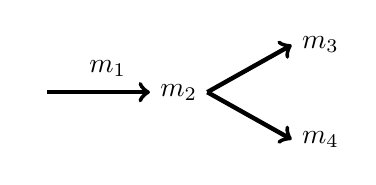
\begin{tikzpicture}[thick,scale=0.6]
\node (1) at (-3,0) {};
\node (2) at (0,0) {$m_2$};
\node (3) at (3,1) {$m_3$};
\node (4) at (3,-1) {$m_4$};
\node (m1) at (-1.5,0.5) {$m_1$};
\draw[arrows={->},ultra thick] (1.east)--(2.west);
\draw[arrows={->},ultra thick] (2.east)--(3.west);
\draw[arrows={->},ultra thick] (2.east)--(4.west);
\end{tikzpicture}
\captionof{figure}{Sistema Laboratorio}
\end{center}
\end{minipage}
\hfill
\begin{minipage}[t]{0.45\linewidth}
\begin{center}
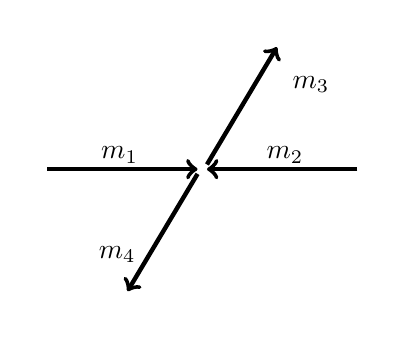
\begin{tikzpicture}[thick,scale=0.6]
\node (1) at (-3.5,0) {};
\node (2) at (3.5,0) {};
\node (3) at (1.8,2.8) {};
\node (4) at (-1.8,-2.8) {};
\draw[arrows={->},ultra thick] (1.east)--(-0.1,0)  ;
\draw[arrows={->},ultra thick] (2.west)--(0.1,0)  ;
\draw[arrows={->},ultra thick] (0.1,0.1)--(3.south west)  ;
\draw[arrows={->},ultra thick] (-0.1,-0.1)--(4.north east)  ;
    
\node (m1) at (-1.75,0.3) {$m_1$};
\node (m2) at (1.75,0.3) {$m_2$};
\node (m3) at (2.3,1.8) {$m_3$};
\node (m4) at (-1.8,-1.8) {$m_4$};
\end{tikzpicture}
\captionof{figure}{Sistema Centro de Masas}
\end{center}
\end{minipage}

\subsubsection{Cálculo de los ángulos}
En esta sección trataremos de obtener los ángulos de salida de las partículas 3 y 4 (y sus energías) en función de las variables conocidas: energía cinética y masas de las partículas. Para esto necesitaremos calcular las energías de las partículas en el sistema centro de masas, ya que las relaciones de conservación de la energía es mucho mas sencilla en este sistema referencial. Luego podremos recuperarlas usando la \textit{transformada de Lorentz}. 

Como podemos ver en las figuras, en el sistema laboratorio la partícula 1 está en movimiento mientras que la partícula 2 está en reposo. Eso nos lleva a que sus momentos, en el sistema de referencia del laboratorio:

\begin{eqnarray}
    P_1 = (E_1/c,\pn_1) & \quad P_2 = (m_2c,0) \\
    P_3 = (E_3/c,\pn_3) & \quad P_4 = (E_4/c,\pn_4)
\end{eqnarray}
Por otro lado, los momentos en el sistema de referencia del centro de masas vendrán dados por

\begin{eqnarray}
    P_1' = (E_1'/c,\pn_1') \quad P_2 = (E_2'/c,-\pn_1') \\ 
    P_3' = (E_3'/c,\pn_3') \quad P_4 = (E_4'/c,-\pn_3')
\end{eqnarray}
Asumiremos que la partícula 1 incidente se mueve únicamente en el eje $x$ tal que $\pn_1=(p_1,0,0)$. En ese caso el sistema centro de masas se moverá respecto al sistema laboratorio en el eje $x$, por lo que habrá que aplicar la transformaciones de Lorentz (\ref{Ec:04} y \ref{Ec:05}) siendo válidas para \textit{cualquier cuadrimomento}. Definimos las energías totales como $E_{tot}=E_1+E_2$ y como  $E_{tot}'=E_1'+E_2'$, siendo esta última la \textit{energía del centro de masas}, que verifica que
\begin{equation}
    E_{tot}' \equiv E_{CM} = E_{tot}^2 - c^2p_1^2 \label{Ec:18}
\end{equation}
Tanto $E_{tot}$ como $E_{tot}'$ son variables conocidas. Nos interesa calcular las energías $E_3'$ y $E_4'$, que usando la transformación de Lorentz nos servirán para estudiar las energías $E_3$ y $E_4$, así como los momentos. Las relaciones se pueden calcular como 

\begin{equation}
    E_c' = E_{tot}' - E_{ex}
\end{equation}
siendo $E_{ex}$ la parte de la energía inicial que se convierte en energía de estados excitados de las partículas 3 y 4. Así pues: 
\begin{eqnarray}
    E_3 ' & = & \frac{1}{2} \left( E_{c}' + \frac{m_3^2c^4- m_4^2c_4}{E_{c}'} \right) \\
    E_4 ' & = & \frac{1}{2} \left( E_{c}' + \frac{m_4^2c^4- m_3^2c_4}{E_{c}'} \right) 
\end{eqnarray}
A partir de estos valores de $E_3'$ y $E_4'$ podemos calcular el valor de los momentos $p_3'$ y $p_4'$ (en módulo). Podemos suponer sin ningún tipo de problema que la coordenada $x$ de los momentos vienen dadas por

\begin{eqnarray}
    p_{3x}' = p_3' \cos (\theta_3') \\
    p_{4x}' = p_4' \cos (\theta_4')
\end{eqnarray}
de este modo podemos aplicar las transformaciones de Lorentz para hallar los valores del $\cos (\theta_3)$ y $\cos (\theta_4)$. Así, usando la ecuación \ref{Ec:09}:

\begin{eqnarray}
    p_3 \cos (\theta_3) = \gamma (p_3' \cos (\theta_3')+\beta E_3'/c)
\end{eqnarray}
despejando $\cos (\theta)$ obtenemos:

\begin{equation}
    \cos (\theta_3) = \frac{\gamma}{p_3} (p_3' \cos (\theta_3')+\beta E_3'/c)
\end{equation}
El cálculo de $p_4$ es exactamente igual, obteniendo


\begin{equation}
    \cos (\theta_4) = \frac{\gamma}{p_4} (p_4' \cos (\theta_4')+\beta E_4'c)
\end{equation}


\subsection{ACTAR TCP}

\subsection{Pérdidas de energía en el Gas}

\subsection{Detectores}


\begin{Anotacion}
    \textcolor{red}{Hay que mencionar los siguientes puntos: 
    \begin{itemize}
        \item Tamaño y resulución
        \item Union PN 
    \end{itemize}
    }
\end{Anotacion}
